\section{Experimentación}

En este apartado se realiza una explicación en profundidad de las pruebas que se han realizado
para validar y verificar la implementación descrita en apartados anteriores. Esta sección incluye
la explicación en detalle de todo el diseño experimental llevado a cabo, incluyendo las técnicas
a comparar, la descripción del \textit{dataset} utilizado para la experimentación, el
procedimiento seguido para realizar el entrenamiento y prueba de los modelos, incluyendo el
\textit{k-fold cross-validation}, la descripción del cálculo de las distintas métricas de
evaluación y, finalmente, los resultados obtenidos y su correspondiente análisis. Además, en esta
última sección, se dará respuesta a las preguntas de investigación planteadas en la Sección
\ref{sec:research_questions}, lo que constituye el objetivo principal de este estudio.

\subsection{Diseño experimental}
\noindent En esta sección se describe el diseño experimental llevado a cabo para la validación
de la implementación propuesta.

\subsubsection{Técnicas a comparar.}
En este estudio, se propone comparar tres técnicas de predicción diferentes. Por un lado, la
propuesta en \textit{SmartBuildSkip} \cite{2} que usa bosques aleatorios en su algoritmo de
predicción y, por otro lado, las dos técnicas propuestas en este estudio, JAES24. A continuación,
se describen las tres técnicas a comparar:

\begin{itemize}
    \item \textbf{SBS-\textit{Within}}: técnica propuesta en \textit{SmartBuildSkip} que utiliza bosques
    aleatorios en su algoritmo de \textit{Machine Learning} para la predicción. Esta técnica
    tiene dos fases principales: una en la que el algoritmo predice de forma automática que
    la \textit{build} fallará, por encontrarse en una secuencia de \textit{build failures}, y
    otra en la que utiliza predicción mediante \textit{Machine Learning}.\\

    \item \textbf{JAES24-\textit{Within}}: técnica propuesta en este estudio que utiliza como modelo de
    ML árboles de decisión. El algoritmo de predicción se basa en la implementación propuesta de
    \textit{SmartBuildSkip}, pero modificando el conjunto de \textit{features} empleado: TF, NC,
    FC, LC, LA, LR, LT, WD y DH, el cual captura eventos temporales al realizar las \textit{builds}
    y desgrana los cambios realizados en la misma. Además, en este algoritmo se realiza la
    acumulación de \textit{features}, lo cual permite acumular cambios para la predicción cuando
    una \textit{build} es saltada por el algoritmo.\\
    
    \item \textbf{JAES24-\textit{Without}}: técnica propuesta en este estudio que utiliza como modelo de
    ML árboles de decisión. Este modelo emplea el mismo conjunto de \textit{features} descrito en
    el punto anterior, sin embargo, no utiliza como base la implementación realizada
    \textit{SmartBuildSkip}, por lo que no se realiza acumulación de valores en las \textit{features}
    cuando una \textit{build} es saltada por el algoritmo, ni tampoco tiene dos fases de predicción.
    En este caso, simplemente se van realizando predicciones de forma individual para cada
    \textit{build}.
\end{itemize}

Dependiendo del contexto sobre el que se realicen las predicciones, puede ser más adecuado
utilizar una técnica u otra. Por ejemplo, si el proyecto sobre el que realizamos predicciones
suele tener muchos \textit{build failures} de forma consecutiva, será más beneficioso utilizar
las técnicas SBS-\textit{Within} o JAES24-\textit{Within}, ya que estas tienen una fase
en la predicción especialmente diseñada para detectar secuencias de \textit{build failures}. Por
otro lado, si el proyecto tiene \textit{build failures} producidos más aleatoriamente a lo largo
del proyecto, será más beneficioso utilizar la técnica JAES24-\textit{Without}, ya que esta no 
tiene en cuenta secuencias de \textit{build failures} en su algoritmo de predicción.\\

Realizar una comparación entre estas tres técnicas nos da una visión más amplia de los
resultados obtenidos en este estudio, permitiéndonos identificar cual de ellas es más adecuada en
términos de precisión, eficiencia o adaptabilidad a las características del problema. El hecho
de considerar varias técnicas mejora la validez interna del estudio, ya que se descarta que los
resultados sean atribuibles a una sola metodología.

\subsubsection{Descripción del \textit{dataset}.}
Para realizar la experimentación, se han utilizado $20$ proyectos de código abierto disponibles
de forma pública en \textit{GitHub}. Todos los proyectos están basados en \textit{Java} y
han sido seleccionados de forma manual. Con el objetivo de tener una experimentación diversa,
se han tenido en cuenta dos escenarios posibles:

\begin{enumerate}
    \item \textbf{Escenario 1}: engloba a todos aquellos proyectos donde la  CI falla con muy
    poca frecuencia. En nuestra solución, se ha considerado a todos estos proyectos como
    ``proyectos difíciles'', y serán todos aquellos en los que la proporción de \textit{build
    failures} es inferior al $10\%$ con respecto a las \textit{builds} exitosas.\\

    \item \textbf{Escenario 2}: engloba a todos aquellos proyectos donde la CI falla con
    una frecuencia ``normal''. Consideramos como ``proyectos normales'' a todos aquellos en los
    que el porcentaje de \textit{build failures} se encuentra comprendido entre el $10\%$ y el
    $25\%$ con respecto a las \textit{builds} exitosas.
\end{enumerate}

Al incluir tanto proyectos difíciles como normales, se pretende obtener una visión más amplia
de la efectividad de nuestro algoritmo en diferentes condiciones y escenarios. Este enfoque
es beneficioso por varias razones:

\begin{itemize}
    \item \textbf{Evaluación en escenarios específicos}: separar ambos escenarios nos permite
    analizar el comportamiento del modelo en cada tipo de proyecto de forma más precisa.\\

    \item \textbf{Fortalezas y debilidades}: al evaluar cada conjunto de proyectos individualmente,
    podemos identificar fortalezas y debilidades del modelo en cada escenario.\\

    \item \textbf{Adaptabilidad del modelo}: al evaluar el modelo en diferentes escenarios, podemos
    observar si el modelo es capaz de adaptarse bien a ambos tipos de proyectos, o si realmente
    necesita un enfoque diferente para cada uno de ellos.
\end{itemize}

Se ha decidido catalogarlos como ``proyectos difíciles'' y ``proyectos normales'' según la
capacidad que tendrá el algoritmo de aprender de los \textit{build failures} en cada tipo de 
proyecto. En los proyectos difíciles, donde se espera que la proporción de \textit{build
failures} sea mucho menor a la de \textit{builds} exitosas, el algoritmo tendrá que aprender
de un número mucho menor de ejemplos de fallos, haciéndole la tarea de aprendizaje más difícil.
Por otro lado, en los proyectos normales, donde la proporción de \textit{build failures} es
más alta, el algoritmo tendrá más ejemplos de \textit{build failures} sobre los que aprender,
esperando que la capacidad de aprendizaje sea mayor.\\

Como hemos mencionado anteriormente, se han seleccionado $20$ proyectos de código abierto
disponibles en \textit{GitHub}. Cada uno de ellos ha sido seleccionado de forma manual, y se
ha intentado que el número de \textit{builds} sea lo más similar posible entre ellos. A
continuación, se muestran dos gráficos que describen la proporción de \textit{build failures}
en cada uno de los proyectos seleccionados, tanto para proyectos difíciles como para proyectos
normales.\\

\begin{figure}[H]
    \centering
    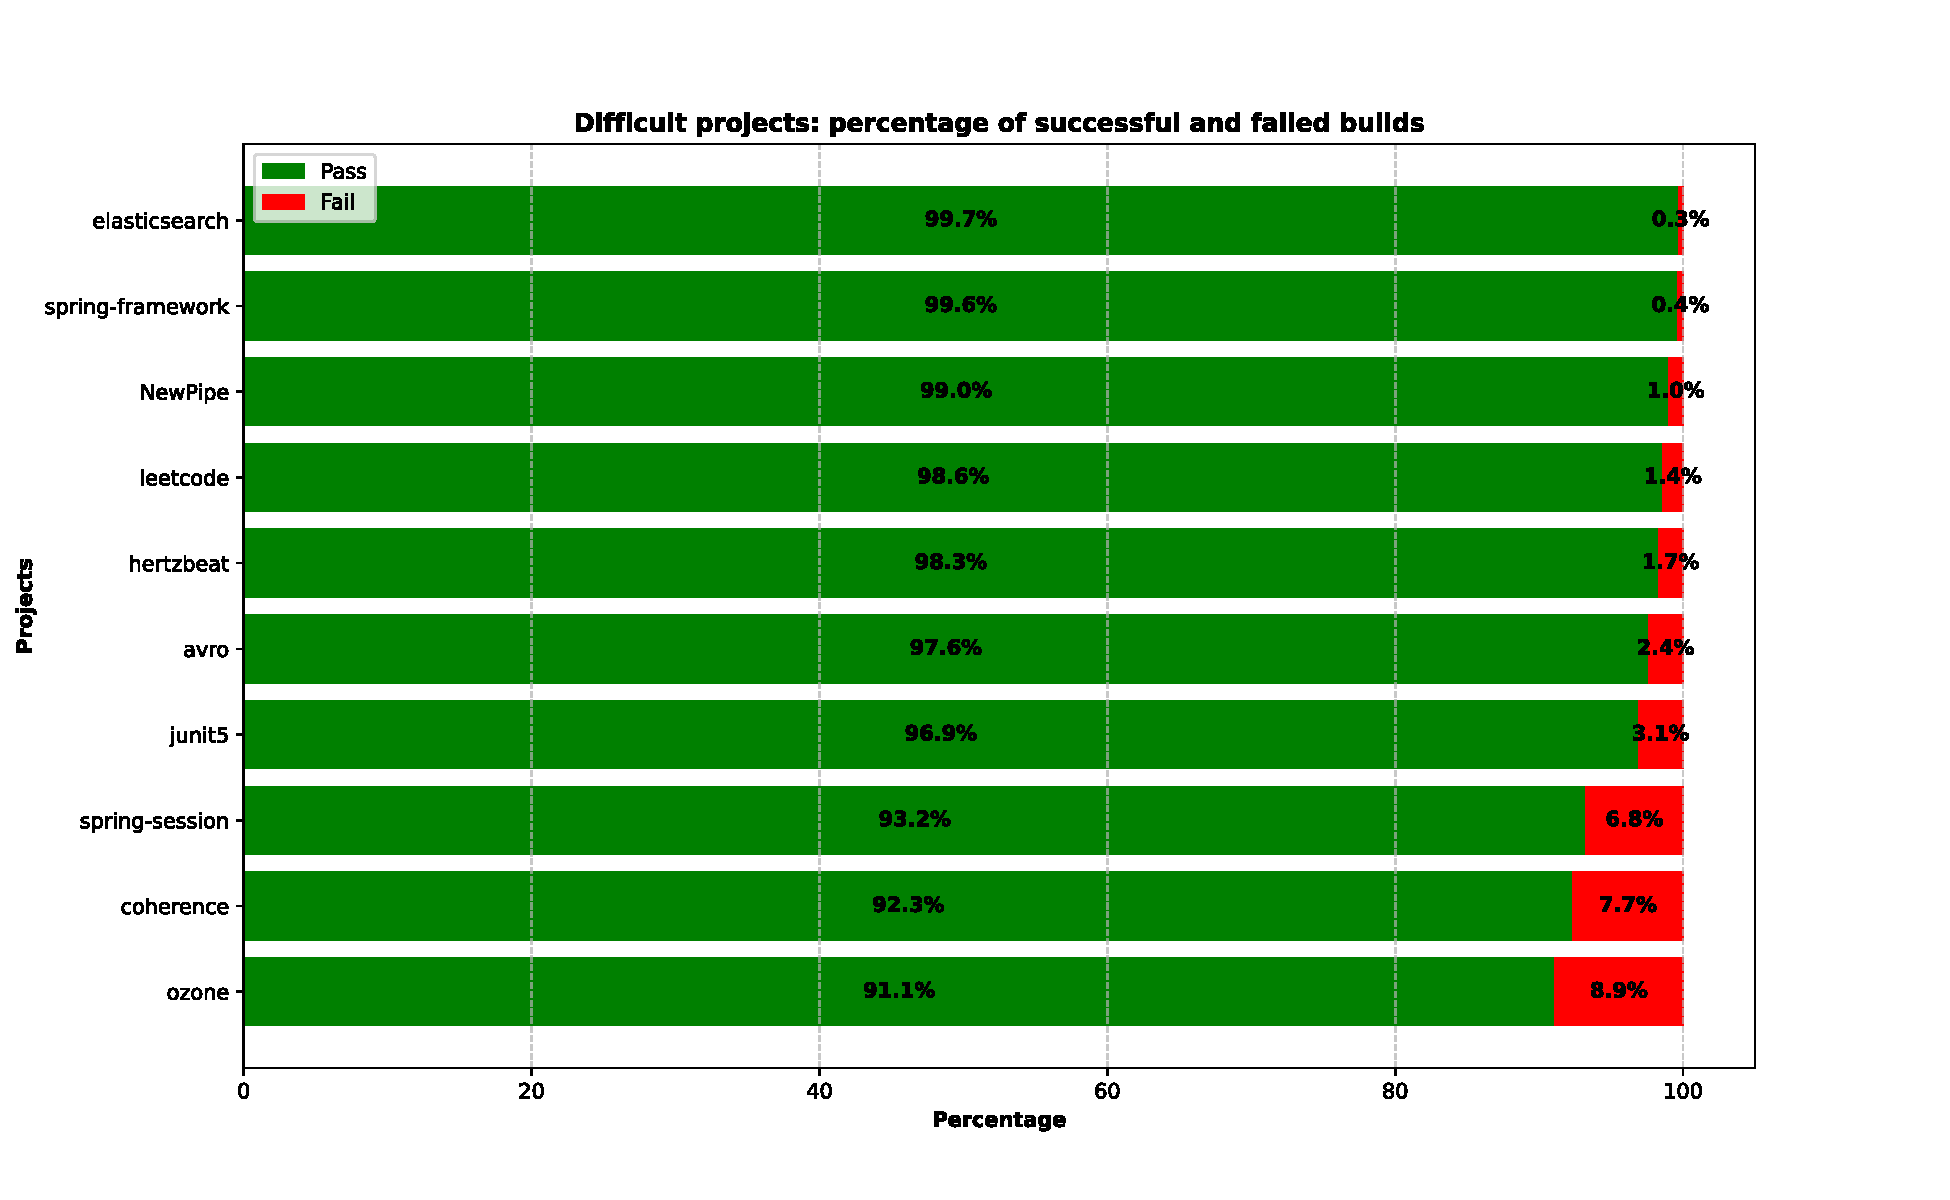
\includegraphics[width=0.85\textwidth]{images/Failures_difficult_projects.pdf}
    \caption{Proporción de \textit{build failures} en proyectos difíciles}
    \label{fig:failures_difficult_projects}
\end{figure}

\begin{figure}[H]
    \centering
    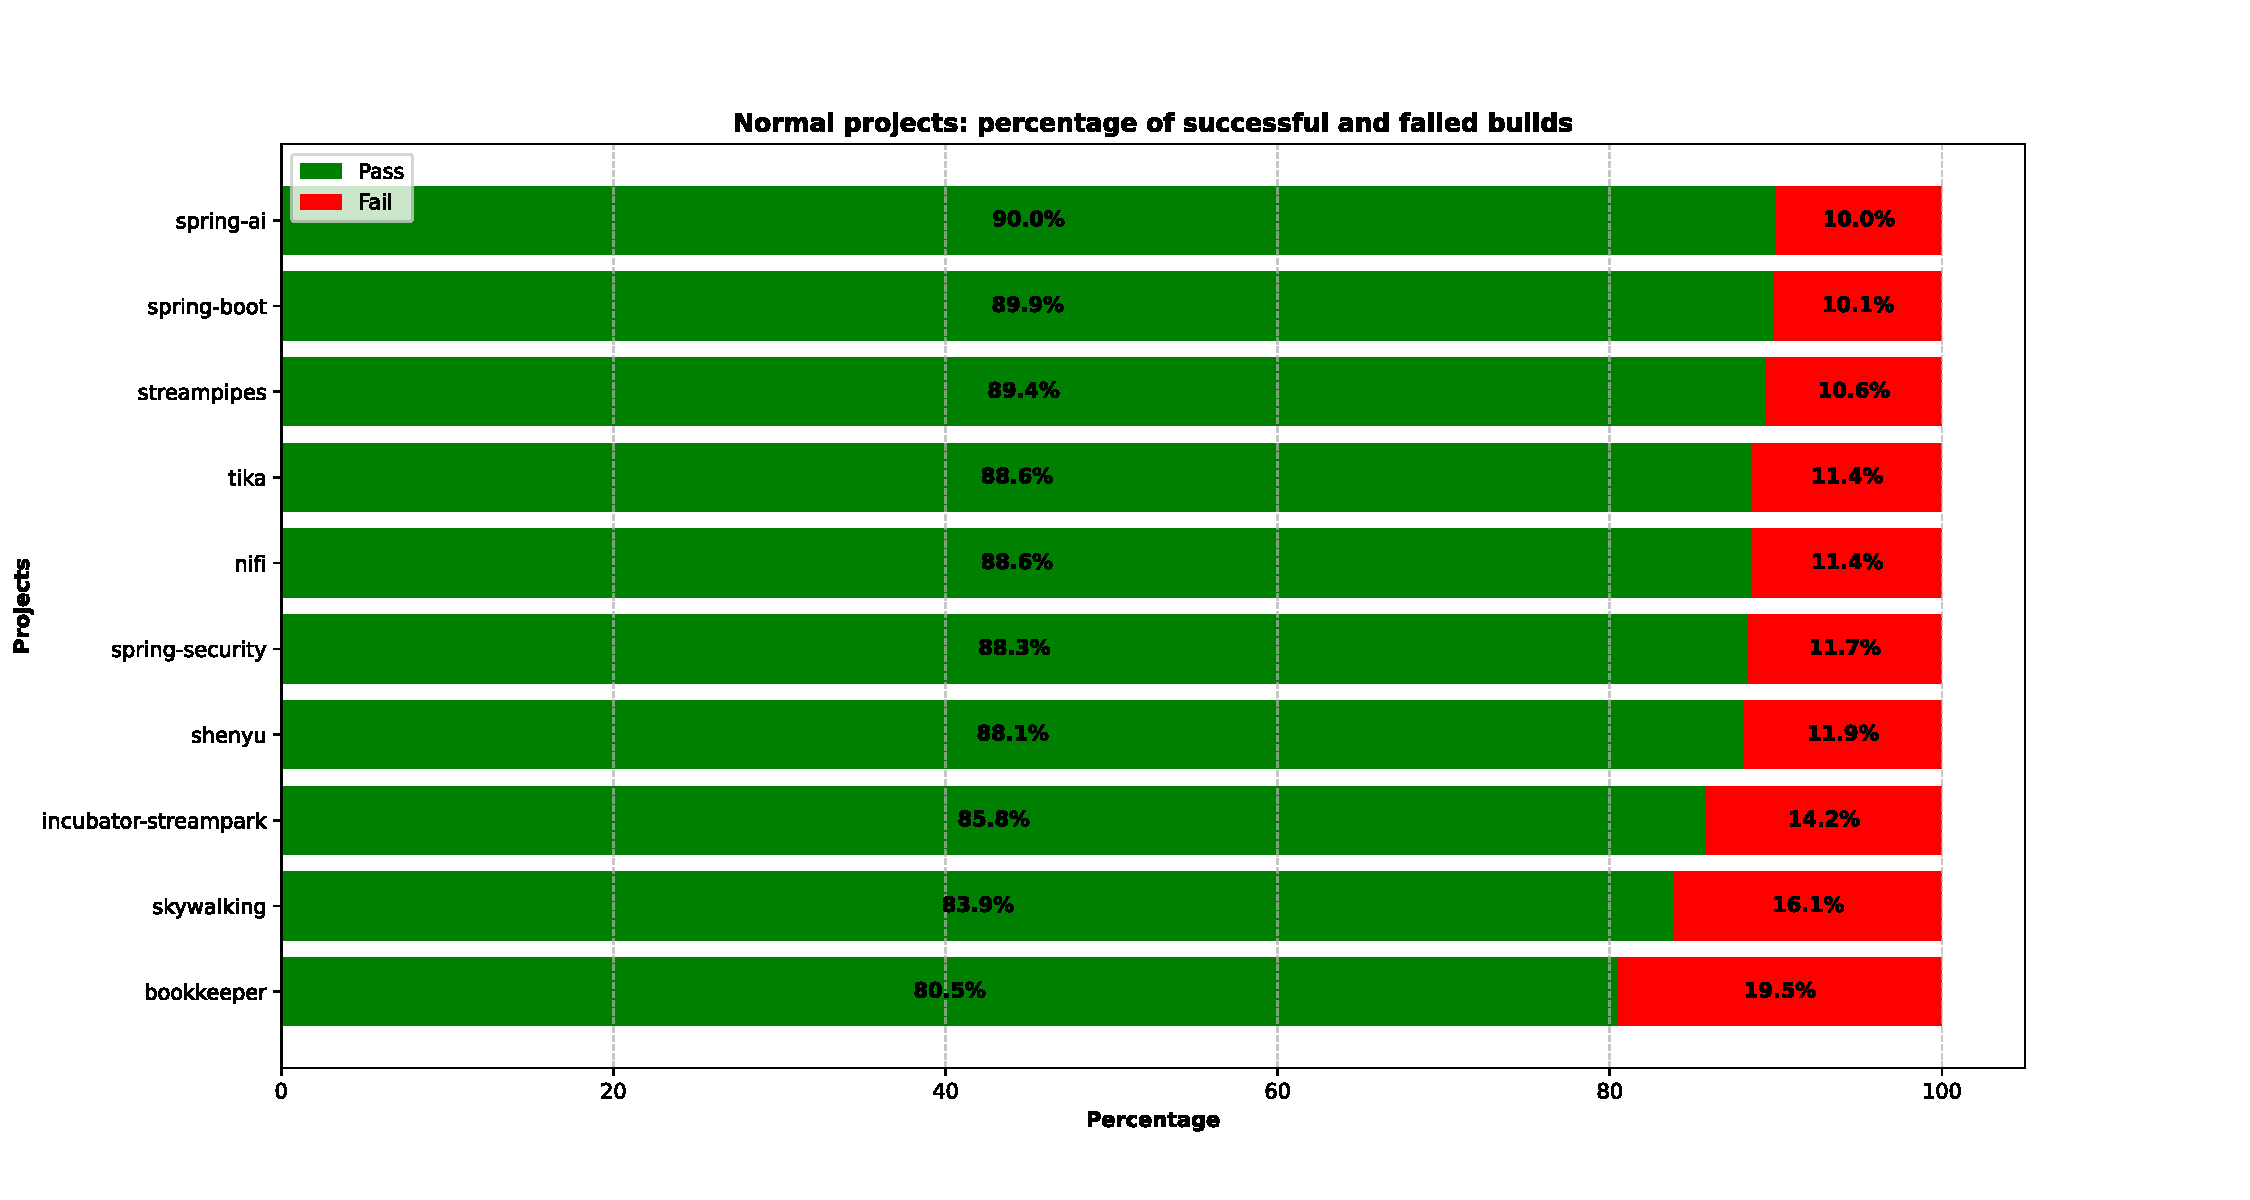
\includegraphics[width=0.85\textwidth]{images/Failures_normal_projects.pdf}
    \caption{Proporción de \textit{build failures} en proyectos normales}
    \label{fig:failures_normal_projects}
\end{figure}

Como vemos, en los proyectos difíciles la proporción de \textit{build failures} es inferior al
$10\%$, mientras que en los proyectos normales se encuentra entre el $10\%$ y el $25\%$. En
ambos casos, se ha intentado que el número de \textit{builds} sea lo más similar posible entre
los proyectos seleccionados.\\

\subsubsection{Procedimiento para el entrenamiento, prueba  y validación cruzada}
La evaluación de los modelos de clasificación busca medir y analizar el desempeño de los mismos
en la tarea de clasificación. Esta evaluación permite determinar la capacidad del modelo para
predecir o clasificar correctamente nuevas instancias no observadas previamente, utilizando un
conjunto de datos de prueba.\\

\noindent Para cada uno de los $20$ proyectos seleccionados, se ha realizado lo siguiente:


\begin{enumerate}
    \item \textbf{Conjunto de entrenamiento y prueba}: se ha dividido el subconjunto de
    \textit{builds} en dos subconjuntos, uno de entrenamiento y otro de prueba. El porcentaje
    de entrenamiento y prueba se ha fijado en $80\%$ y $20\%$ respectivamente. Se ha tenido
    especial cuidado en seleccionar el $80\%$ de las \textit{builds} más antiguas para el
    subconjunto de entrenamiento y, el $20\%$ de las \textit{builds} más recientes para el
    subconjunto de prueba. Esto es así por la dependencia temporal que existe en este tipo de
    problemas, donde no tiene sentido realizar predicciones basándonos en información futura.
    Además, para realizar este entrenamiento y prueba, se ha escogido el umbral de decisión
    por defecto, con valor $0.5$.\\

    \item \textbf{K-fold cross-validation}: se ha utilizado la técnica de validación cruzada
    \textit{k-fold cross-validation} para evaluar el rendimiento de los modelos de clasificación
    propuestos. Para cada proyecto, se han seleccionado sus \textit{builds} y se han creado $11$
    subconjuntos a partes iguales. A continuación, se ha realizado la validación cruzada de
    la siguiente forma: se han ido seleccionando los \textit{folds} de forma acumulativa para
    realizar el entrenamiento, mientras que con el \textit{fold} siguiente se ha realizado la
    parte de \textit{test}. Cuando este proceso se ha realizado con cada uno de los \textit{folds},
    habrá un total de $10$ resultados disponibles, calculando así posteriormente la media de cada
    una de las métricas obtenidas en cada \textit{fold}. Este proceso se ha realizado
    con un umbral de decisión de $0.5$, con el fin de contrastar los resultados obtenidos para el 
    conjunto de entrenamiento y prueba.\\
\end{enumerate}

\subsubsection{Métricas de evaluación}
Las métricas de evaluación constituyen una parte esencial en nuestro estudio, ya que gracias a
ellas podemos medir y analizar el rendimiento de las técnicas propuestas. En este estudio, se
han considerado cinco métricas de evaluación diferentes: \textit{accuracy}, \textit{precision},
\textit{recall}, \textit{F1-score} y \textit{AUC-ROC}. Estas métricas ya fueron descritas en la
Sección \ref{sec:research_questions}, por lo que no se describirán de nuevo en este apartado.\\


Es importante mencionar que, para realizar el cálculo de estas métricas, hemos hecho uso de
métodos de la librería \textit{metrics} de \textit{scikit-learn}. Esta librería está especialmente
diseñada para el cálculo de estas métricas, y nos permite obtener los resultados de forma
rápida y sencilla. A continuación, vamos a describir cómo se realiza el cálculo de cada una de
ellas en el procedimiento de \textbf{entrenamiento y prueba}:

\begin{itemize}
    \item \textit{Accuracy}: a partir de las predicciones realizadas por el modelo para el
    conjunto de \textit{test} (que supone el $20\%$ de las \textit{builds}), se calcula a
    partir de los valores de las etiquetas reales de las \textit{builds} y las predicciones
    realizadas por el modelo (Ecuación \eqref{eq:accuracy}).\\

    \item \textit{Precision}: a partir de las etiquetas reales del conjunto de \textit{test} y
    las etiquetas predichas por el algoritmo, se calcula la precisión del modelo
    (Ecuación \eqref{eq:precision}). Hemos tenido que indicar cuál es la clase positiva en nuestro problema
    (clase 0) e incluir el valor por defecto que asigna cuando se produce una división entre $0$,
    en el caso de que la suma de verdaderos positivos y falsos positivos sea $0$.\\

    \item \textit{Recall}: a partir de las etiquetas reales del conjunto de \textit{test} y las
    etiquetas predichas por el algoritmo, se calcula el \textit{recall} del modelo
    (Ecuación  \eqref{eq:recall}). Al igual que en el caso de \textit{precision}, hemos tenido que indicar
    cuál es la clase positiva en nuestro problema (clase 0) para que el cálculo sea correcto y,
    añadir el valor por defecto en caso de división entre $0$, en este caso, cuando la suma de
    verdaderos positivos y falsos negativos sea $0$.\\

    \item \textit{F1-score}: esta métrica, podría calcularse directamente a partir de los valores
    de \textit{precision} y \textit{recall}, sin embargo, hemos decidido utilizar el método que
    nos proporciona la librería mencionada anteriormente, que usa al igual que los anteriores las
    etiquetas reales del conjunto de \textit{test} y las etiquetas predichas por el algoritmo,
    además de indicar cuál es la clase positiva y el valor en caso de división entre $0$.\\
\end{itemize}

En el caso de \textbf{\textit{k-fold cross-validation}}, el cálculo en sí de estas métricas
es similar al descrito anteriormente, con la característica de que por cada \textit{fold} de
\textit{test} evaluado, se almacenan las predicciones, hasta que finalmente se tengan los
resultados de $k-1$ \textit{folds}, en este caso $10$ folds. Una vez obtenidos estos resultados,
estos serían las etiquetas predichas por el algoritmo.

\begin{figure}[H]
    \centering
    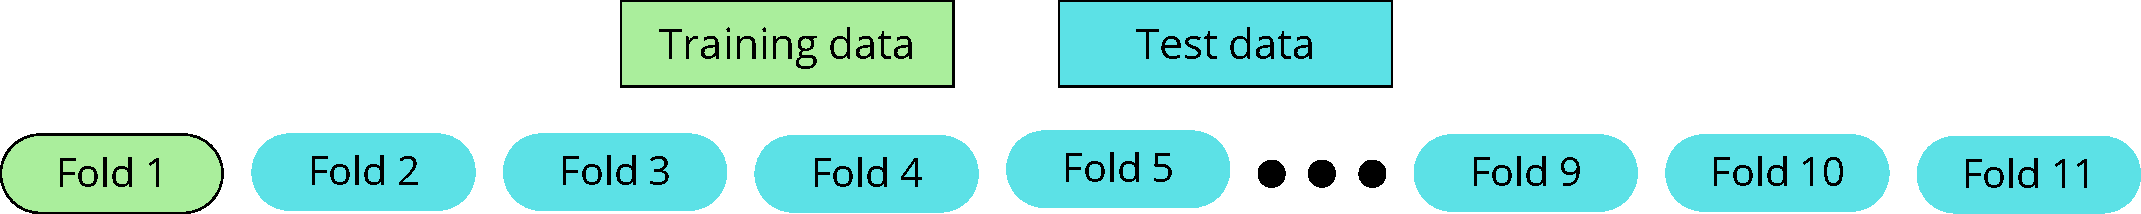
\includegraphics[width=0.9\textwidth]{images/Folds predictions.pdf}
    \caption{Acumulación de predicciones en \textit{k-fold cross-validation}.}
    \label{fig:fold-predictions}
\end{figure}

Como vemos en la Figura \ref{fig:fold-predictions}, hemos ido acumulando las predicciones hechas
en cada uno de los \textit{folds} de \textit{test}, para luego calcular las métricas en función
de ellas. Podemos observar, además, que el primer \textit{fold} no se usa para \textit{test},
usándose únicamente para entrenamiento. Sucede algo similar con el último \textit{fold}, que no
es usado para entrenamiento y se usa únicamente para \textit{test}.\\

\subsection{Resultados}
En este apartado, se presentan los resultados obtenidos del estudio y se responde a las
preguntas de investigación planteadas en la Sección \ref{sec:research_questions}. A continuación,
se presentan con detalle las pruebas realizadas y el análisis de los resultados obtenidos.\\

\begin{mdframed}[backgroundcolor=gray!10,linewidth=0.5pt,roundcorner=1pt]
    \textbf{PI-1:} ¿Qué algoritmo de predicción produce los mejores resultados en la predicción automática del re-
    sultado de la integración continua?
\end{mdframed}

Para responder a esta pregunta de investigación, se ha realizado un análisis comparativo entre
las tres técnicas presentadas, cada uno de los cuales ha sido evaluado en los dos escenarios
posibles: proyectos difíciles y proyectos normales. 

\subsubsection{Escenario 1 - Proyectos difíciles.} Evaluación comparativa de las tres técnicas
mediante entrenamiento y prueba, $80\%$ y $20\%$ respectivamente, con un umbral de decisión
de $0.5$, el valor por defecto.\\

\begin{figure}[H]
    \centering
    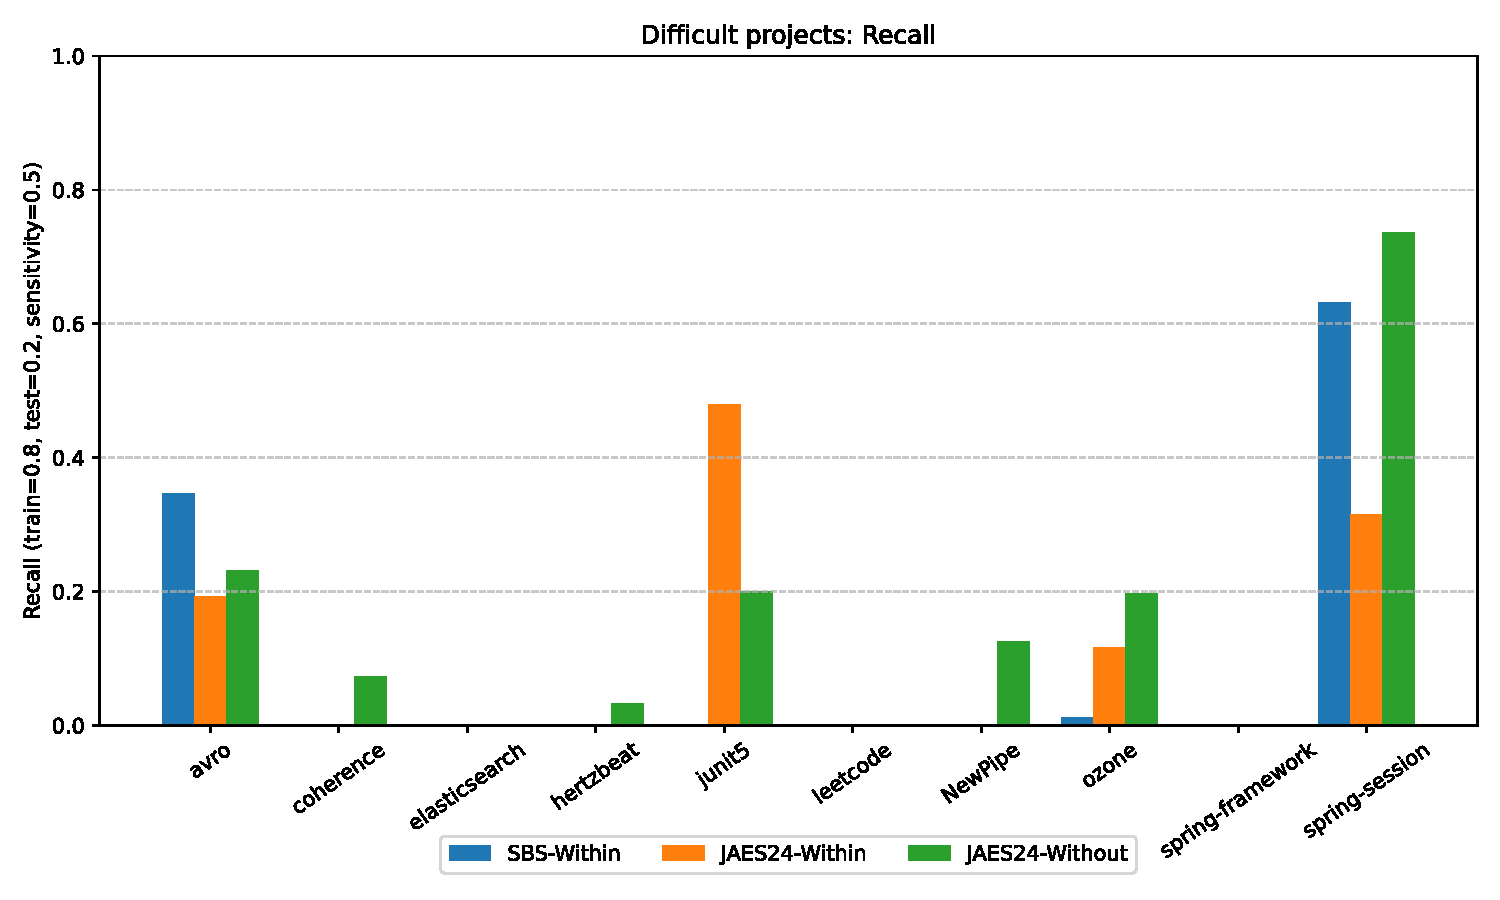
\includegraphics[width=0.7\textwidth]{images/Difficult projects: Recall.pdf}
    \caption{\textit{Recall} en proyectos difíciles}
    \label{fig:train_test_recall_difficult_projects}
\end{figure}

En la Figura \ref{fig:train_test_recall_difficult_projects}, podemos observar los valores de
\textit{recall} obtenidos en los proyectos difíciles. Como vemos, no se han obtenido valores
demasiado altos, sin embargo, en prácticamente todos los proyectos, JAES24 ha obtenido
mejores resultados que \textit{SmartBuildSkip}. A simple vista, parece que JAES24-\textit{Without}
ofrece mejores valores de \textit{recall}, ya que en proyectos como \textit{coherence},
\textit{hertzbeat} o \textit{NewPipe} es el único que consigue predecir algún \textit{build
failure}. En otros, como en \textit{ozone} y \textit{spring-session}, es superior. Observando
la gráfica, podemos ver que en \textit{avro} se obtienen mejores valores para SBS-\textit{Within},
esto puede deberse a que en este proyecto las \textit{features} que usa SBS-\textit{Within} 
sean más significativas que en otros proyectos, aunque por lo general, JAES24-\textit{Without}
es el que mejor se comporta.\\

\begin{figure}[H]
    \centering
    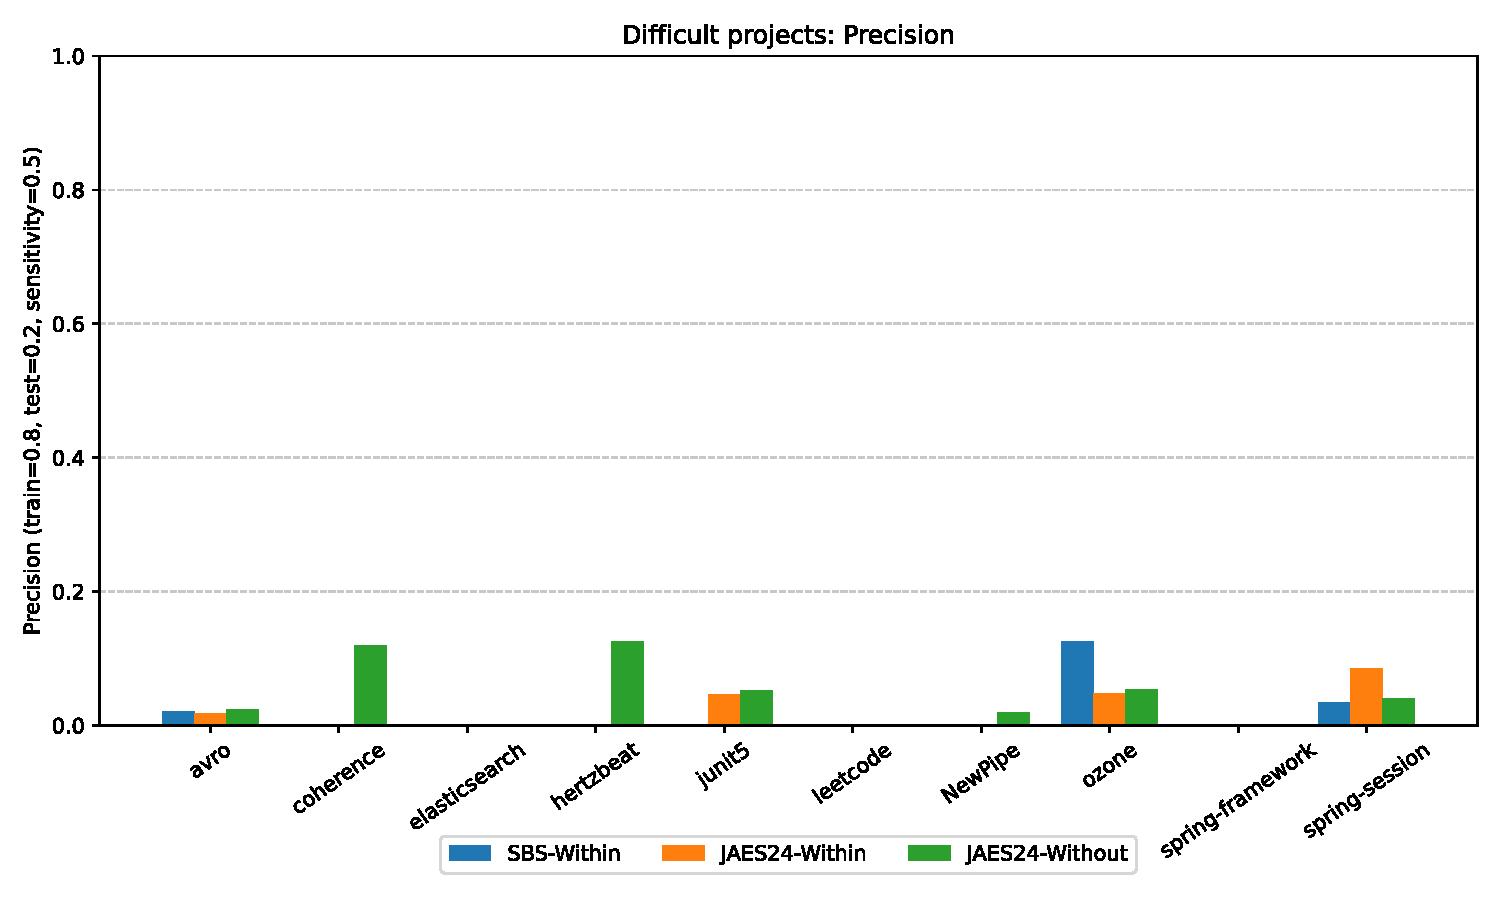
\includegraphics[width=0.7\textwidth]{images/Difficult projects: Precision.pdf}
    \caption{\textit{Precision} en proyectos difíciles.}
    \label{fig:train_test_precision_difficult_projects}
\end{figure}

En este caso, tenemos que el \textit{precision} es bastante bajo para las tres técnicas, sin
embargo, JAES24 ofrece resultados ligeramente superiores que \textit{SmartBuildSkip}.
Actualmente, el modelo se equivoca prediciendo como \textit{build failures} una cantidad elevada
de \textit{builds} que en realidad no lo son. Debemos recordar que, en este escenario, el modelo
tiene muy pocas instancias positivas de las que aprender, haciendo este proceso de aprendizaje
más complicado. Aún así, JAES24-\textit{Without} es el que mejor se comporta en este aspecto.\\

Con el fin de validar los resultados obtenidos y clarificar cuál de las técnicas de JAES24
es la que mejor se comporta, vamos a realizar las mismas gráficas usando \textbf{\textit{k-fold
cross-validation}} en lugar de \textit{train} y \textit{test}. Esta validación cruzada ha sido
realizada usando un umbral de decisión de $0.5$ y $11$ particiones.

\begin{figure}[H]
    \centering
    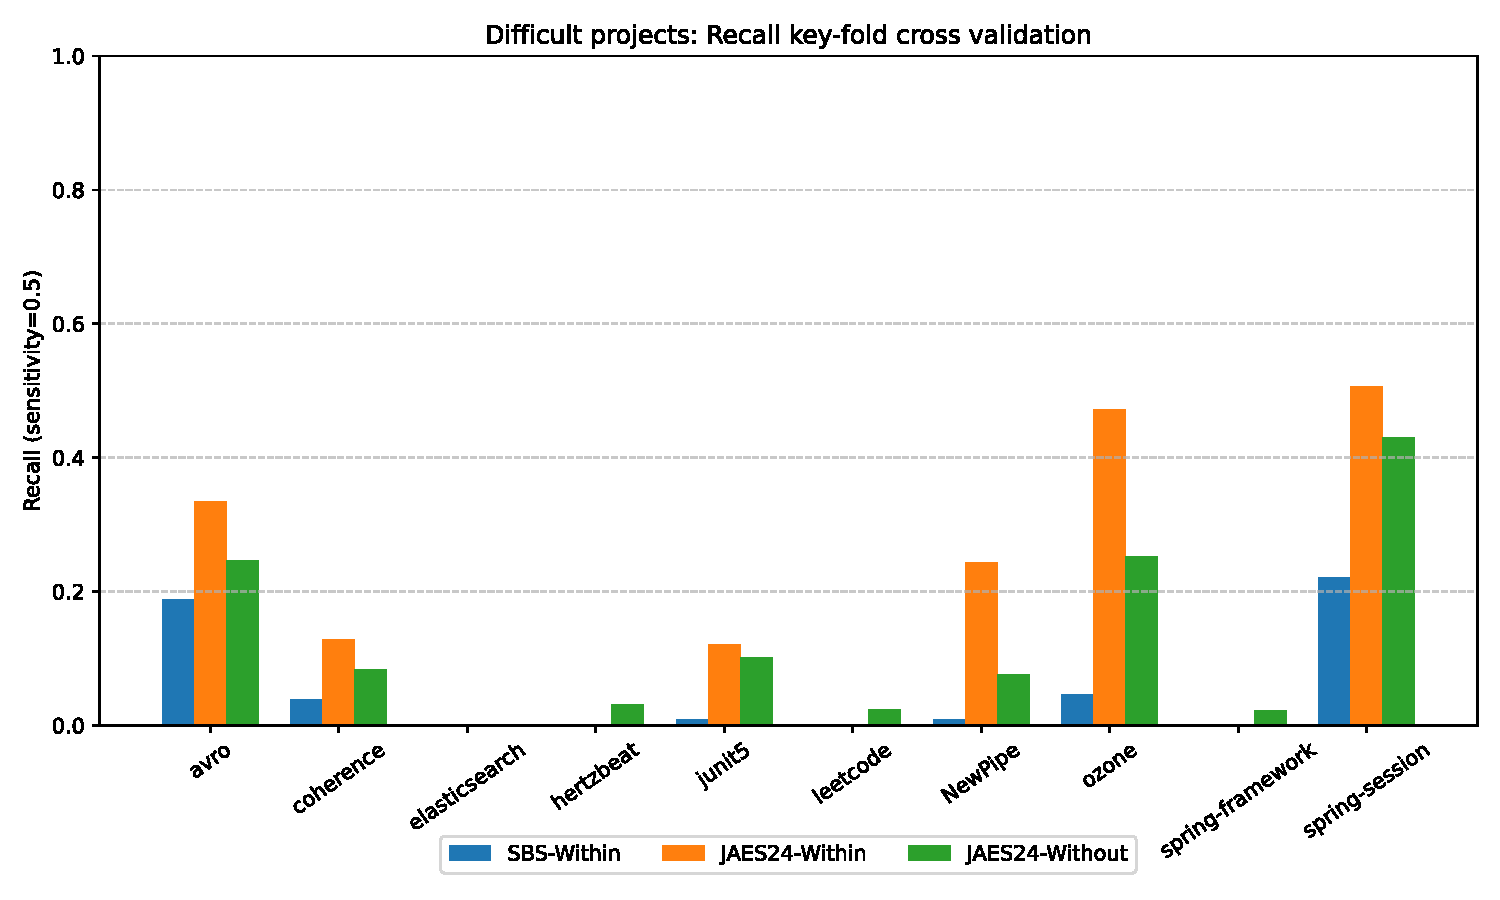
\includegraphics[width=0.7\textwidth]{images/Difficult projects: Recall key-fold cross validation.pdf}
    \caption{\textit{Recall} en proyectos difíciles usando validación cruzada.}
    \label{fig:key-fold_recall_difficult_projects}
\end{figure}

Tras realizar validación cruzada sobre nuestro \textit{dataset} de proyectos difíciles, podemos
observar en la Figura \ref{fig:key-fold_recall_difficult_projects} que los resultados varían
ligeramente a los anteriores. En este caso, se observa claramente que JAES24-\textit{Within} es
la que mejor resultados obtiene en cuando a \textit{recall}. Ambas técnicas, tanto
JAES24-\textit{Within} como JAES24-\textit{Without}, ofrecen mejores resultados que
\textit{SmartBuildSkip}. Si comparamos únicamente las técnicas de JAES24, podemos deducir
que JAES24-\textit{Within} se comporta mejor en este \textit{dataset} de proyectos porque
probablemente exista un mayor número de \textit{build failures} de forma consecutiva, lo cual no
quiere decir que JAES24-\textit{Without} sea peor, simplemente que en este contexto, JAES24-\textit{Within}
se comporta mejor.\\

\begin{figure}[H]
    \centering
    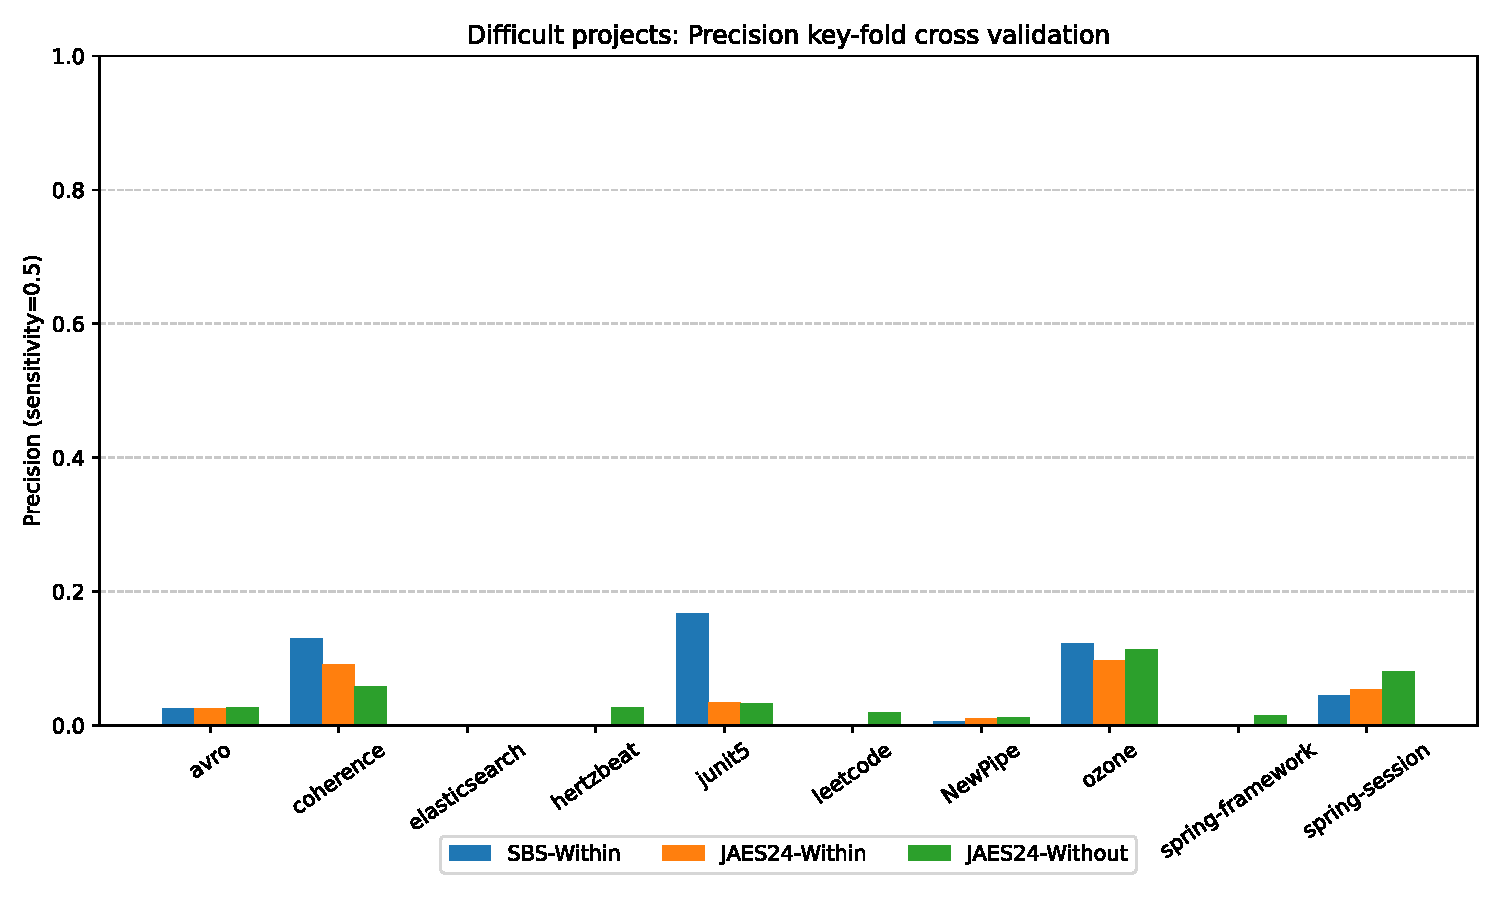
\includegraphics[width=0.7\textwidth]{images/Difficult projects: Precision key-fold cross validation.pdf}
    \caption{\textit{Precision} en proyectos difíciles usando validación cruzada.}
    \label{fig:key-fold_precision_difficult_projects}
\end{figure}

En la Figura \ref{fig:key-fold_precision_difficult_projects}, podemos observar resultados algo
contradictorios, ya que en algunos casos SBS-\textit{Within} ofrece mejores resultados para
el \textit{precision}, mientras que en otros, JAES24-\textit{Without} es el que mejor se comporta.
Sin embargo, en más de la mitad de los proyectos seleccionados, JAES24-\textit{Without} es el que
mejores resultados ofrece para \textit{precision}.\\

Si nos fijamos, a pesar de que JAES24-\textit{Within} ofrezca mejores resultados en \textit{recall},
JAES24-\textit{Without} es el que mejor se comporta en \textit{precision}. Esto nos parece
adelantar dos variantes del algoritmo muy interesantes:

\begin{itemize}
    \item JAES24-\textit{Within}: se trata de una técnica más agresiva para identificar fallos. Si
    el desarrollador quiere asegurarse de predecir la mayor cantidad de fallos (aunque esto
    implique ejecutar \textit{builds} que en realidad no fallarán), esta técnica es la más
    adecuada.\\

    \item JAES24-\textit{Without}: es una técnica más conservadora, pero cuando predice un fallo,
    es más probable que sea correcto. Si el objetivo del desarrollador es minimizar falsas
    alarmas y tener predicciones más confiables, esta técnica es más adecuada.
\end{itemize}

La decisión de utilizar una u otra técnica dependerá de las necesidades del proyecto y del
desarrollador. Si la prioridad es detectar el mayor número de fallos posibles, incluso a costa de
más falsos positivos, JAES24-\textit{Within} es la mejor opción. Si la prioridad es minimizar
falsas alarmas y asegurar que cuando se predice un fallo, realmente ocurra, entonces
JAES24-\textit{Without} es la mejor opción.\\


\subsubsection{Escenario 2 - Proyectos normales.} Evaluación comparativa de las tres técnicas
mediante entrenamiento y prueba, $80\%$ y $20\%$ respectivamente, con un umbral de decisión
de $0.5$, el valor por defecto.

\begin{figure}[H]
    \centering
    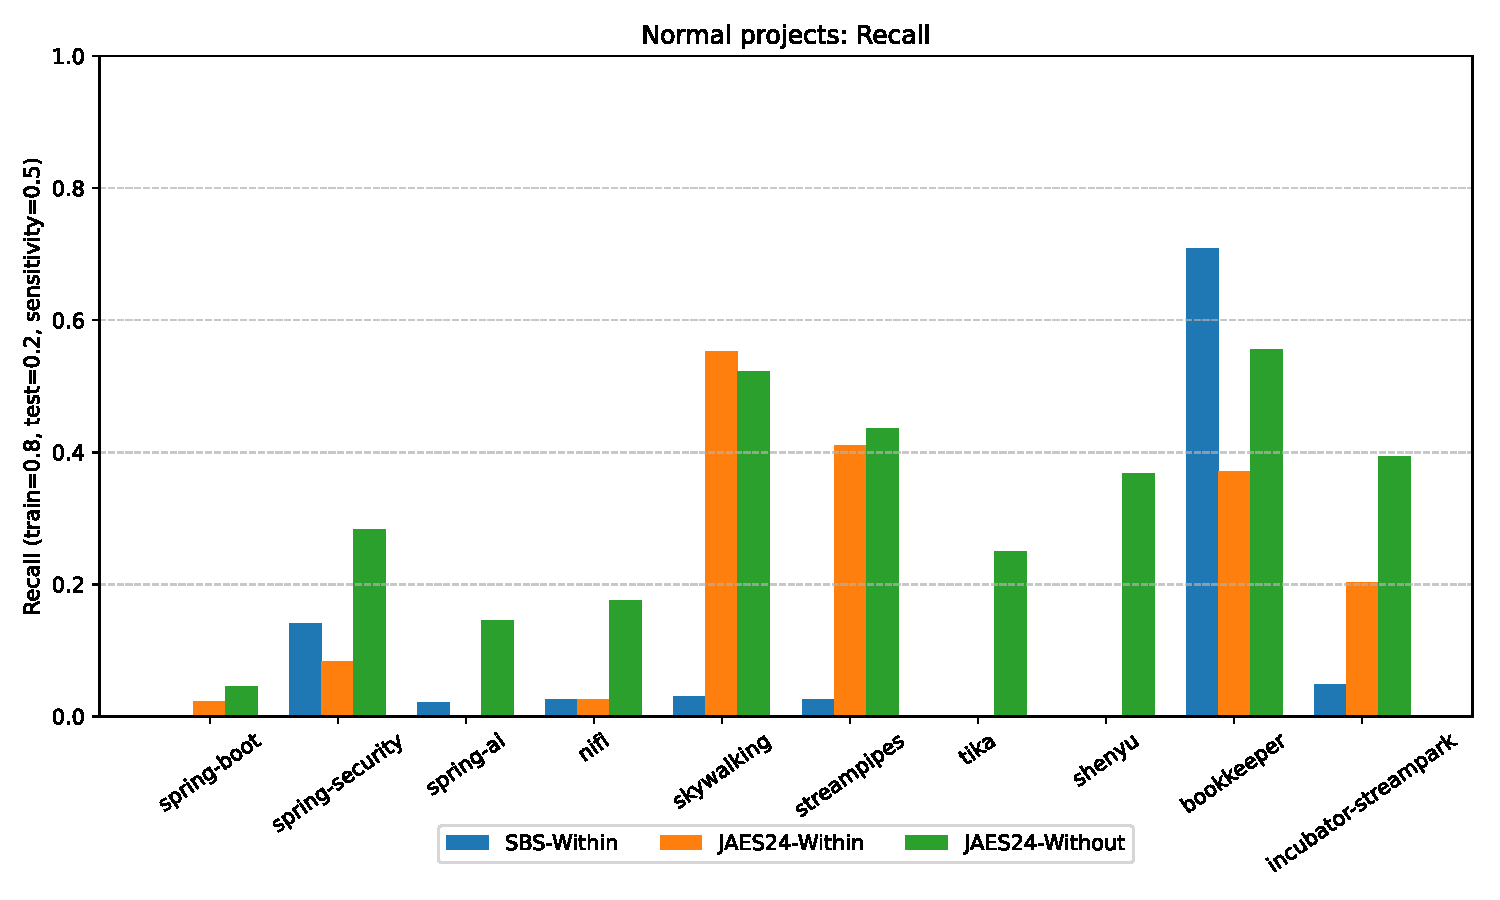
\includegraphics[width=0.7\textwidth]{images/Normal projects: Recall.pdf}
    \caption{\textit{Recall} en proyectos normales.}
    \label{fig:train_test_recall_normal_projects}
\end{figure}

Observando los resultados obtenidos en la Figura \ref{fig:train_test_recall_normal_projects},
vemos que las tres técnicas se comportan mucho mejor que en el Escenario $1$. En este caso,
los modelos tienen una mayor cantidad de \textit{build failures} sobre los que aprender, lo que
hace más sencillo el proceso de aprendizaje. A simple vista, parece que JAES24-\textit{Without}
es la que mejor resultados ofrece, siendo superior el \textit{recall} en ocho de los diez
proyectos evaluados. En el proyecto \textit{skywalking}, vemos que JAES24-\textit{Within} ofrece
mejores resultados y, en el proyecto \textit{bookkeeper}, el que mayor número de \textit{build
failures} posee, SBS-\textit{Within} es el que mejor se comporta. Por lo general, vemos que
JAES24, en cualquiera de sus dos variantes, ofrece mejores resultados que
\textit{SmartBuildSkip}.

\begin{figure}
    \centering
    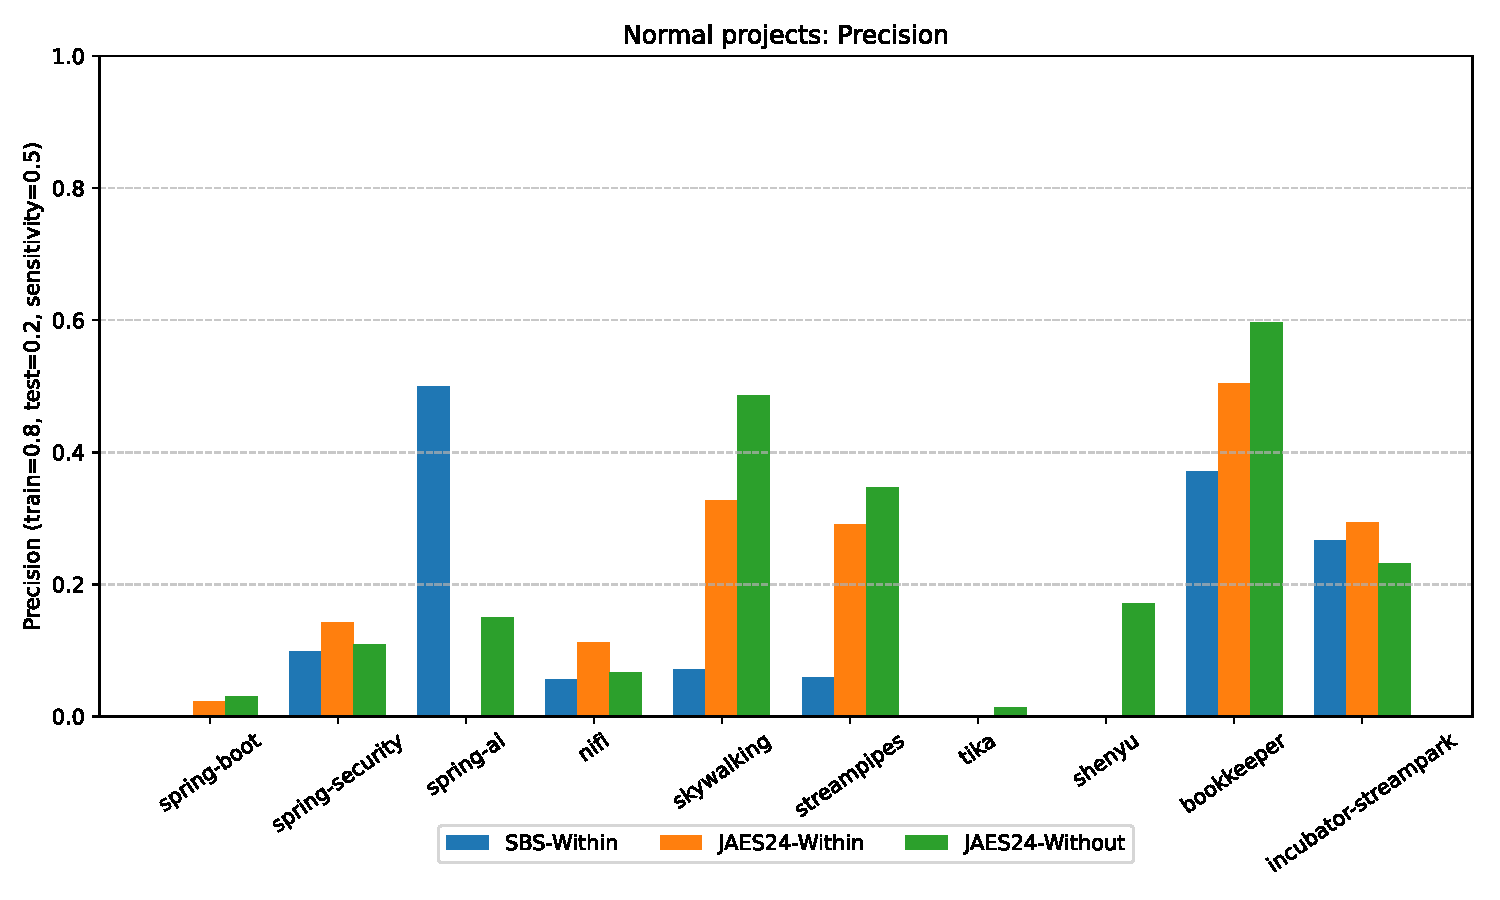
\includegraphics[width=0.7\textwidth]{images/Normal projects: Precision.pdf}
    \caption{\textit{Precision} en proyectos normales.}
    \label{fig:train_test_precision_normal_projects}
\end{figure}

Analizando los resultados de \textit{precision} obtenidos en la Figura
\ref{fig:train_test_precision_normal_projects}, vemos que JAES24-\textit{Without} es el que mejor
resultados ofrece, siendo superior en seis de los diez proyectos evaluados. En otros casos, como
en \textit{spring-security}, \textit{nifi} e \textit{incubator-streampark} es superior 
JAES24-\textit{Within}. Este comportamiento indica que JAES24-\textit{Within} es más preciso
a la hora de predecir \textit{build failures} en los proyectos mencionados anteriormente, es decir, 
predice menor cantidad de falsos positivos que JAES24-\textit{Without}.\\

Con el objetivo de evaluar el rendimiento de manera más robusta y confiable, se ha realizado
\textit{k-fold cross-validation} también en este escenario. Esto evita el sobreajuste y
garantiza que los resultados no dependan únicamente de una partición específica del conjunto
de datos. Para realizar una comparación justa entre escenarios, se ha realizado con el mismo
umbral de decisión, $0.5$ y, con $11$ particiones.

\begin{figure}[H]
    \centering
    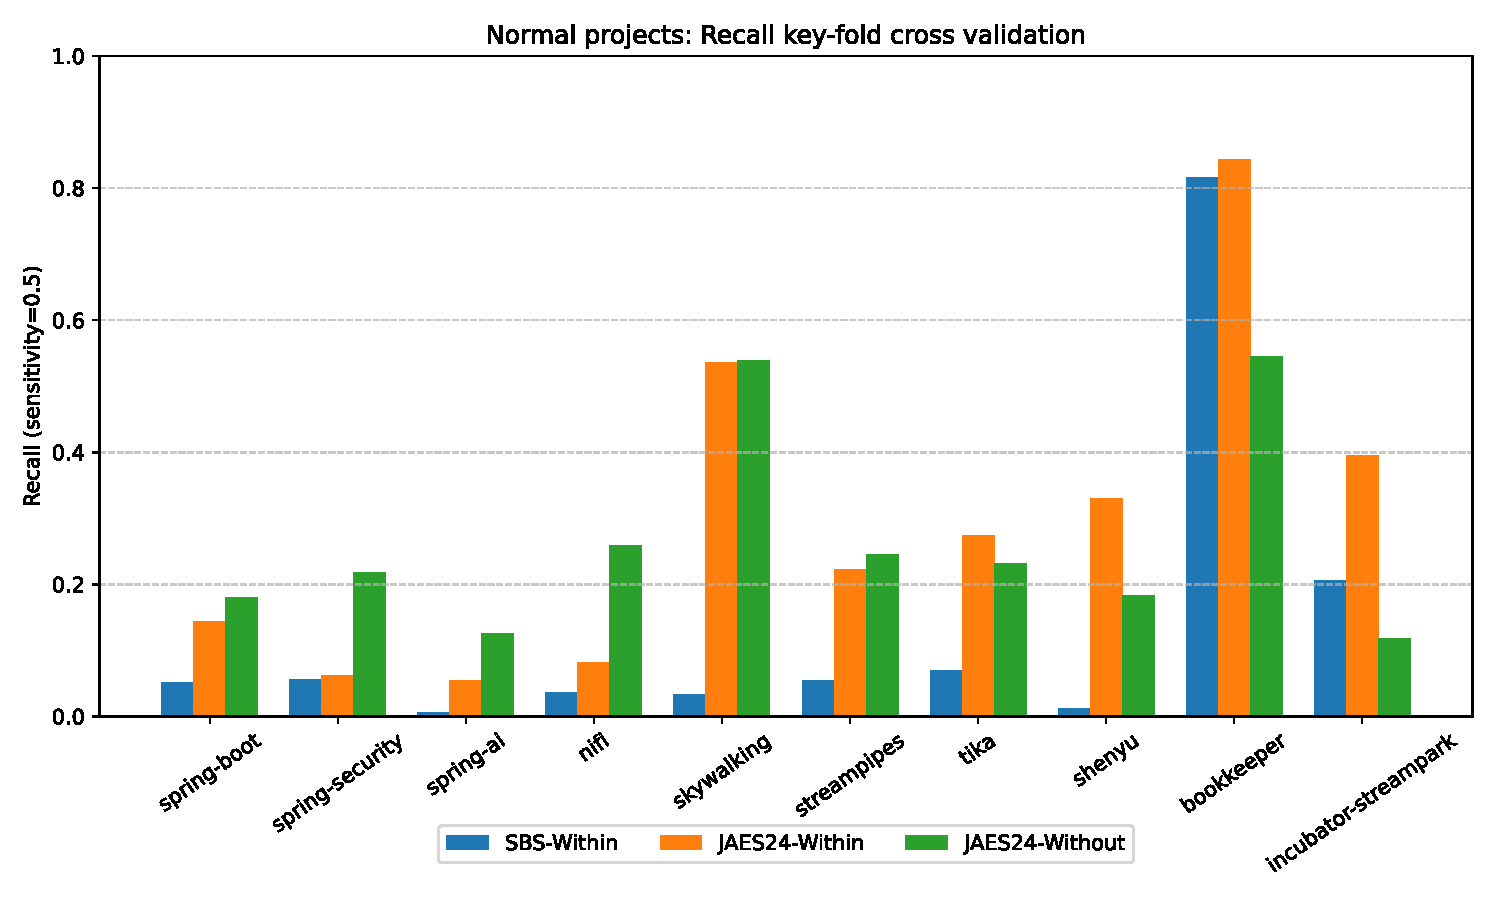
\includegraphics[width=0.7\textwidth]{images/Normal projects: Recall key-fold cross validation.pdf}
    \caption{\textit{Recall} en proyectos normales usando validación cruzada.}
    \label{fig:key-fold_recall_normal_projects}
\end{figure}

Observando los resultados obtenidos en la Figura \ref{fig:key-fold_recall_normal_projects}, vemos
que se obtienen resultados bastante superiores a \textit{SmartBuildSkip}, siendo este enfoque
mucho más efectivo en escenarios donde el número de \textit{build features} es más elevado. Podemos
ver claramente como en casi todos los proyectos (salvo uno) los valores de \textit{recall} de
JAES24 superan a \textit{SmartBuildSkip}. Realizando una comparación entre las técnicas
de JAES24, en los seis primeros proyectos, \textit{JAES-Without} detecta mayor número
de \textit{build failures}, mientras que en los cuatro restantes, JAES24-\textit{Within} ofrece
mejores resultados.\\

Esto nos vuelve a confirmar que la elección de una u otra técnica puede depender de los hábitos
de CI del proyecto. Si en el proyecto detectamos que normalmente se producen fallos
de forma consecutiva, será más apropiado utilizar como técnica de predicción
JAES24-\textit{Within}, ya que esta garantiza que al encontrar un primer fallo (\textit{first
failure}), se prediga de forma automática que la siguiente \textit{build} no pasará. En cambio,
si detectamos que normalmente los \textit{build failures} se producen de forma más aleatoria en
el conjunto de \textit{builds}, será más apropiado utilizar JAES24-\textit{Without}.

\begin{figure}[H]
    \centering
    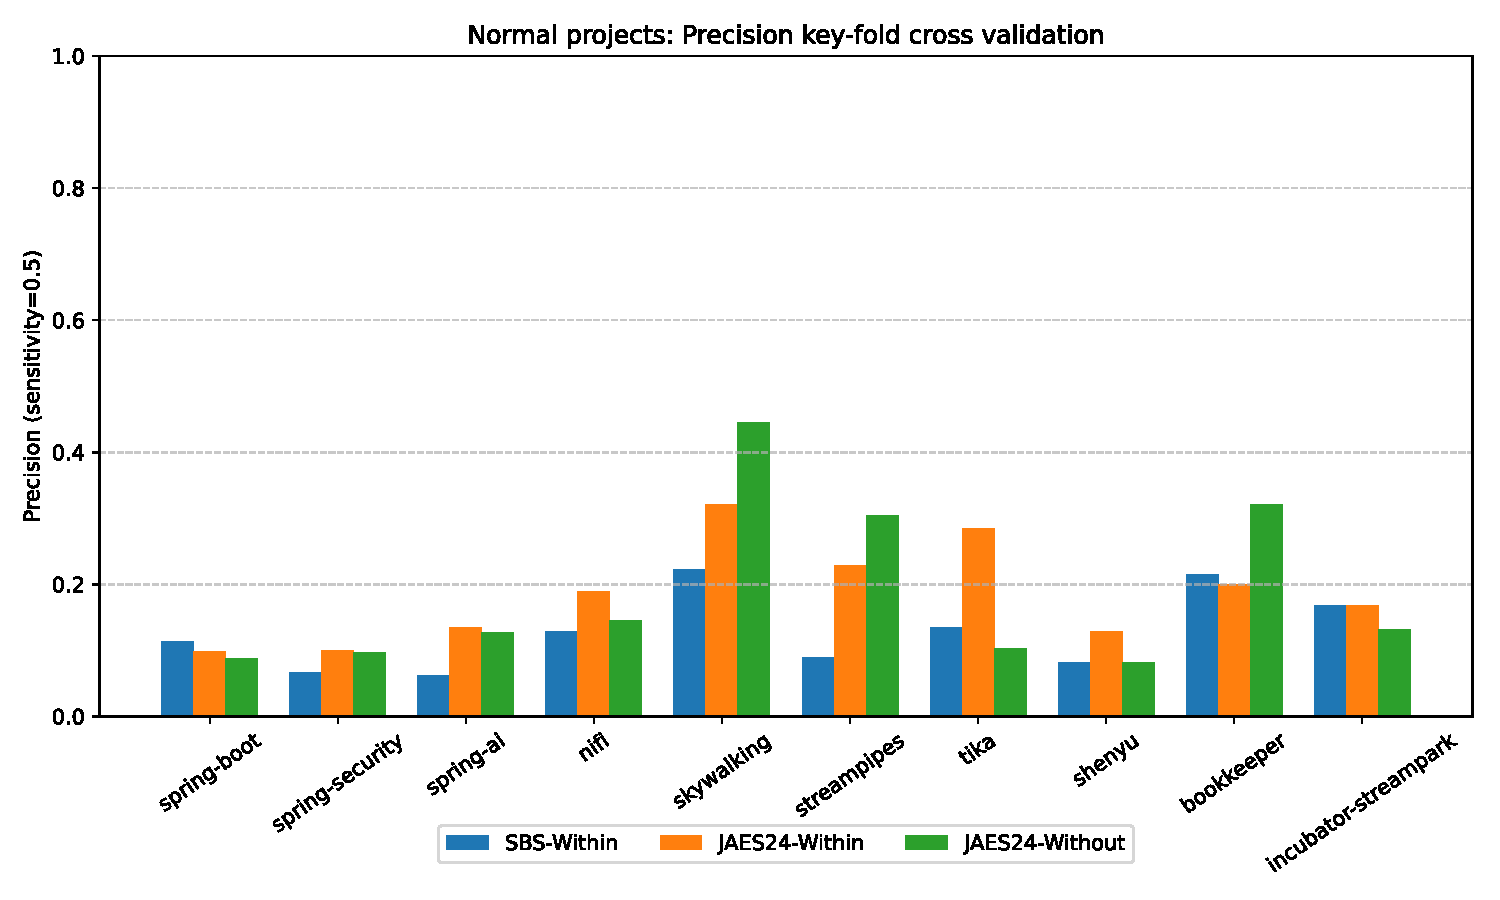
\includegraphics[width=0.7\textwidth]{images/Normal projects: Precision key-fold cross validation.pdf}
    \caption{\textit{Precision} en proyectos normales usando validación cruzada.}
    \label{fig:key-fold_precision_normal_projects}
\end{figure}

Finalmente, en la Figura \ref{fig:key-fold_precision_normal_projects}, vemos que se produce una
tendencia algo distinta a la observada en el Escenario $1$. En este caso, vemos que igualmente
ambas técnicas superan a \textit{SmartBuildSkip}, sin embargo, JAES24-\textit{Within} es la que
mejores resultados ofrece en cuanto a \textit{precision}, siendo superior en siete de los diez
proyectos evaluados. Por lo tanto, tenemos que en este \textit{dataset} de proyectos normales, la
técnica JAES24-\textit{Within} es más conservadora, ya que ofrece menos \textit{recall} a cambio
de aumentar el \textit{precision} y, JAES24-\textit{Without} es más agresiva, ya que ofrece más
\textit{recall} a cambio de disminuir el \textit{precision}.\\

Los resultados obtenidos en este apartado confirman que las \textit{features} que capturan el
\textbf{\textit{timing} en el que se quiere realizar la contribución} (\textit{Time Frequency},
\textit{Week Day} y \textit{Day Hour)}, y las \textbf{\textit{features} que desgranan los cambios
realizados} en la \textit{build} (\textit{Lines Added} y \textit{Lines Removed}) son más
significativas que otras \textit{features} evaluadas en otras técnicas \cite{2}. Estas
características ofrecen una mayor capacidad predictiva, lo que sugiere que el momento en el que
se ejecuta la \textit{build} y el tipo de modificaciones introducidas tienen un impacto directo
en la probabilidad de que se produzcan \textit{build failures}. Este hallazgo subraya la
importancia de considerar, no solo aspectos técnicos del código, sino también el contexto temporal
y la naturaleza de los cambios realizados.\\

\begin{mdframed}[backgroundcolor=gray!10,linewidth=0.5pt,roundcorner=1pt]
    \textbf{PI-2:} ¿Qué características de las builds son más significativas en la predicción?
\end{mdframed}

Para responder a esta pregunta de investigación, hemos aplicado un enfoque basado en el análisis
de importancia de características, utilizando dos algoritmos de clasificación diferentes:
árboles de decisión y bosques aleatorios, que son los usados por las dos técnicas propuestas en
este estudio de JAES24 y, \textit{SmartBuildSkip}, respectivamente. Para ello, hemos
considerado el conjunto completo de \textit{features} disponibles de la Tabla \ref{tab:features}
y hemos calculado la importancia de cada una de ellas para cada proyecto. Posteriormente, hemos
calculado la media de la importancia de cada \textit{feature} en cada algoritmo de clasificación,
obteniendo así una visión general de cuáles son las \textit{features} más significativas en la
predicción.\\

\noindent A continuación, se presentan los valores medios de importancia de cada \textit{feature}
para árboles de decisión:

\begin{figure}[H]
    \centering
    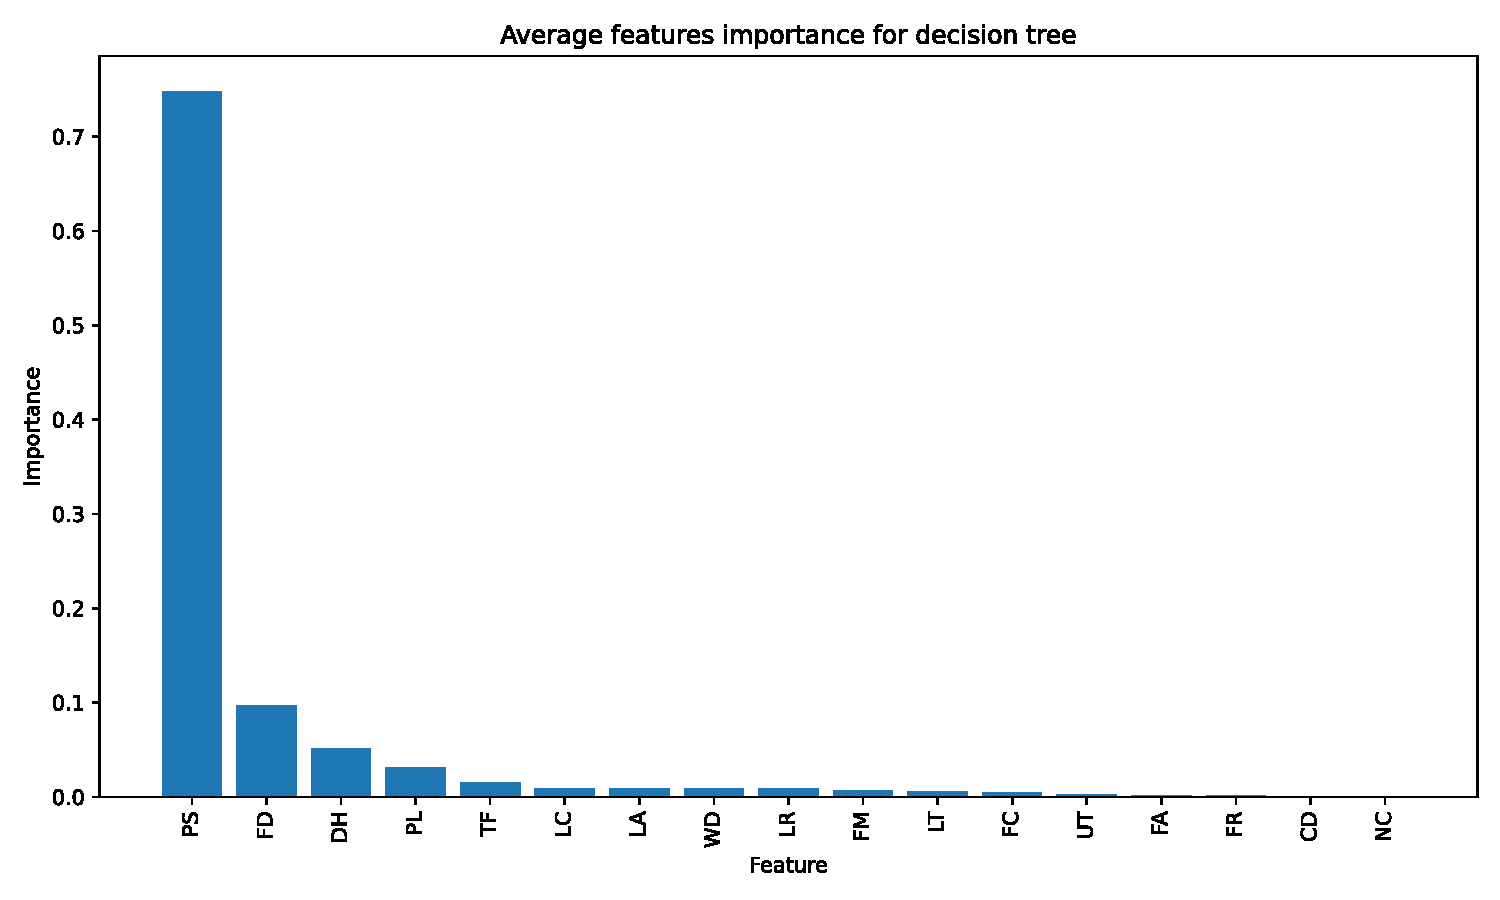
\includegraphics[width=0.7\textwidth]{images/Average features importance for decision tree.pdf}
    \caption{Importancia de las \textit{features} en árboles de decisión.}
    \label{fig:decision_tree_feature_importance}
\end{figure}

\noindent A continuación, se presentan los valores medios de importancia de cada \textit{feature}
para bosques aleatorios:

\begin{figure}[H]
    \centering
    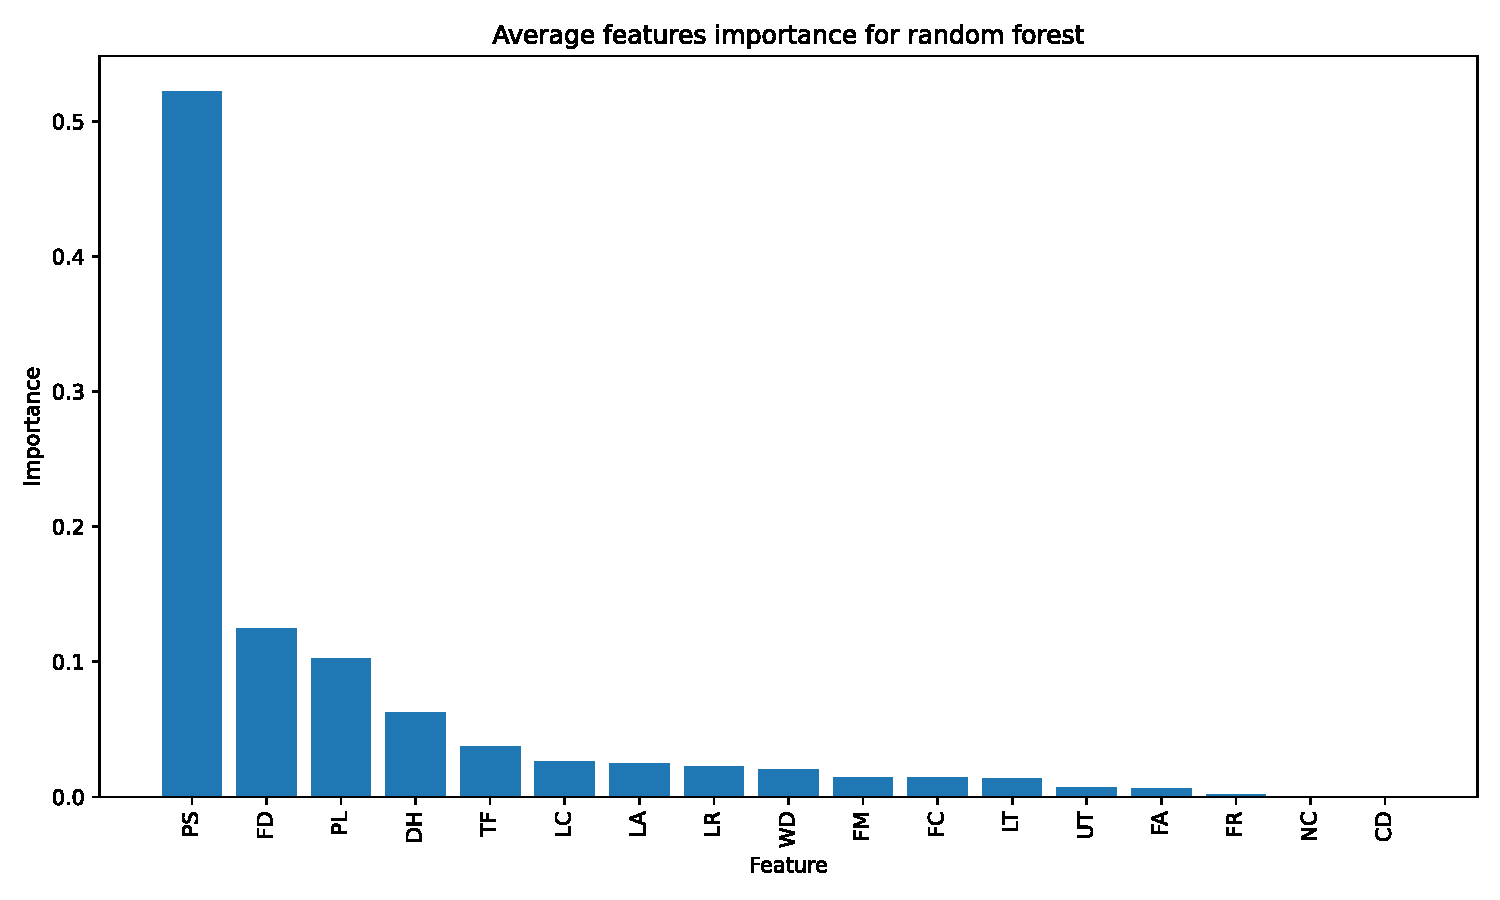
\includegraphics[width=0.7\textwidth]{images/Average features importance for random forest.pdf}
    \caption{Importancia de las \textit{features} en bosques aleatorios.}
    \label{fig:random_forest_feature_importance}
\end{figure}

\noindent Considerando todas las \textit{features} del conjunto presentado en la Tabla \ref{tab:features},
observamos lo siguiente:

\begin{itemize}
    \item Cuando se realiza el entrenamiento del modelo, las \textit{features} que tienen relación
    con el histórico de \textit{builds} ejecutadas anteriormente, como \textit{Performance short},
    \textit{Failure Distance} y \textit{Performance Long}, tienen una importancia significativa
    a la hora de predecir \textit{build failures}.\\

    \item Las \textit{features} que describen el \textit{timing} en el que se realiza la
    contribución como el \textit{Day Hour}, \textit{Time Frequency} y \textit{Week Day} tienen
    una importancia significativa en la predicción de \textit{build failures}.\\

    \item Las \textit{features} que describen los cambios realizados, como \textit{Lines changed}
    y otras que desgranan los cambios realizados en la \textit{build}, como \textit{Lines Added}
    y \textit{Lines Removed}, son también importantes en la predicción de \textit{build failures}.
\end{itemize}

Cabe destacar que, apesar de que las \textit{features} que más importancia tienen a la hora de
predecir \textit{build failures} son el PS, PL y FD, estas \textit{features} no se han utilizado
en nuestro enfoque. Esto se debe a que, en un caso de uso real, si nos encontramos utilizando
un modelo predictivo para decidir si saltar o no una \textit{build}, estas \textit{features} no
podrán calcularse de forma exacta, ya que no conocemos el resultado de aquellas \textit{builds}
propuestas que se hayan predicho como \textit{pass}. En nuestra implementación, se ha realizado
experimentación añadiendo este conjunto de \textit{features}, pero los resultados obtenidos eran
francamente peores que los obtenidos sin ellas. El hecho de asumir que, cuando el algoritmo predice
una \textit{build} propuesta como \textit{pass}, esta realmente lo será (Sección
\ref{sec:features_used}), no ofrece garantías de que el modelo sea efectivo en un caso de uso
real para la predicción.\\

Podemos concluir que, las \textit{features} PL, PS y FD son las que
más influencia tienen a la hora de predecir \textit{build failures}, sin embargo, no son del
todo aplicables a la hora de realizar una predicción en un caso de uso real. Por otro lado, vemos
que \textit{features} que describen el \textit{timing} en el que se realiza la contribución y
las que describen los cambios realizados, son también importantes para la predicción, confirmando
una vez más nuestra hipótesis inicial.\\

Finalmente, con el objetivo de contrastar los resultados y confirmar nuestra hipótesis inicial,
veamos la distribución temporal de \textit{build failures} en el conjunto de repositorios
estudiados:

\begin{table}[H]
    \centering
    \caption{Distribución temporal de los \textit{build failures}.}
    \label{tab:distribution_build_failures}

    \begin{tabular}{|>{\centering\arraybackslash}m{3cm}|>{\centering\arraybackslash}m{3cm}|>{\centering\arraybackslash}m{3cm}|>{\centering\arraybackslash}m{3cm}|} % Encabezados centrados
        \hline
        \textbf{\textit{Día de la semana}} & \textbf{\textit{Builds} ejecutadas} & \textbf{\textit{Builds} fallidas} & \textbf{Proporción de \textit{builds} fallidas}\\
        \hline
        Lunes & 18222 & 836 & 4.59\%\\
        \hline
        Martes & 17447 & 853 & 4.89\%\\
        \hline
        Miércoles & 16690 & 825 & 4.94\% \\
        \hline
        Jueves & 16687 & 877 & 5.26\%\\
        \hline
        Viernes & 15043 & 818 & 5.44\%\\
        \hline
        Sábado & 7510 & 420 & 5.59\%\\
        \hline
        Domingo & 7235 & 376 & 5.19\%\\
        \hline
    \end{tabular}
\end{table}

Estos resultados confirman nuestra hipótesis inicial de que el \textit{timing} en el que se quiere
realizar la contribución juega un papel importante para la predicción de \textit{build failures}.
En la Tabla \ref{tab:distribution_build_failures} podemos observar que la proporción de \textit{build
failures} producidos va aumentando conforme avanza la semana, siendo el viernes y el sábado los dos
días en los que se producen más fallos en comparación con la cantidad de \textit{builds} ejecutadas.
Esto puede deberse posiblemente a la prisa de los desarrolladores por completar las tareas antes
del fin de semana o por la fatiga acumulada durante la semana laboral.

\begin{table}[H]
    \centering
    \caption{Horas en las que se producen más \textit{build failures} para cada día.}
    \label{tab:day_hour_build_failures}

    \begin{tabular}{|>{\centering\arraybackslash}m{3cm}|>{\centering\arraybackslash}m{3cm}|} % Encabezados centrados
        \hline
        \textbf{\textit{Día de la semana}} & \textbf{Hora}\\
        \hline
        Lunes & 12:00\\
        \hline
        Martes & 18:00\\
        \hline
        Miércoles & 18:00\\
        \hline
        Jueves & 18:00\\
        \hline
        Viernes & 18:00\\
        \hline
        Sábado & 18:00\\
        \hline
        Domingo & 18:00\\
        \hline
    \end{tabular}
\end{table}

En la Tabla \ref{tab:day_hour_build_failures}, podemos observar la hora para cada uno de
los días de la semana en que se producen más \textit{build failures}. En este caso, vemos que la
mayoría de fallos tienen lugar a las 18:00 de la tarde, lo cual puede ser bastante razonable,
ya que es normalmente el final de la jornada laboral y, muchos sistemas de CI están configurados
para lanzar las \textit{builds} al final del día laboral. Además, normalmente, los desarrolladores
suelen esperar al final de la jornada para ejecutar la CI, evitando tener que esperar al resultado
de la ejecución de la misma. Por último, observamos que para los lunes, las 12:00 de la mañana es
cuando se producen más fallos, lo cual puede deberse a cambios no ejecutados o menos revisados de
la semana anterior, aunque las razones concretas requieren una mayor investigación.\\
